%% ID: weigh_sea
%% TITLE: Weighing at sea
%% TYPE: question
%% QUESTIONTYPE: numerical
%% CONCEPTS: shm
%% VIDEOS: 
%% LEVEL: 4
%% TOPIC: mechanics/shm
%% ORDER: 10

%Physics: NII, SHM, period, omega
%Maths: trig, trig calculus
\begin{problem}[IntA1985PSIIIQ1p] %Numerical value T = 10s removed, question is now algebraic instead of numerical
{\exposition{A man is standing on a weighing machine on a ship which is pitching up and down with simple harmonic motion of period \vari{T}.} \question{Assuming the motion is vertical calculate the amplitude of the ship's motion in terms of \vari{T}, if the scale reading of the machine varies between limits of \quantity{55}{kg} and \quantity{65}{kg}.}
}
{\textit{Used with permission from UCLES, A Level Physical Science, November 1985, Paper 3, Question 1.3.}}
{Consider the forces acting on the man when he stands on the weighing machine, as in Figure \ref{fig:SHM_man_ship}. The scale's reading depends on the reaction force \vari{R} on the man from the scale; this force varies as the ship moves up and down, while the man's weight remains constant. By symmetry, the man's mass must be midway between the limits given by the scale, so his mass \value{m}{60}{kg}.
\begin{figure}
	\centering
	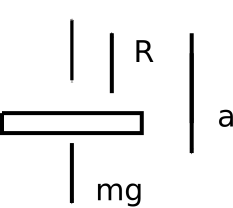
\includegraphics[width=0.25\textwidth]{SHM_man_ship}
	\caption{}
	\label{fig:SHM_man_ship}
\end{figure}

\nl Applying Newton's second law:
\begin{equation*}
60g - R = 60a
\end{equation*}
We know that \vari{a} is at a maximum where the scale reading is at a minimum - i.e.\vari{R} is at a minimum, so the net force acting downwards is at a maximum. As the scale automatically divides the reaction force by \vari{g}, if the minimum scale reading is \quantity{55}{kg} then the minimum \valuedef{R}{55g}{}.
\begin{equation*}
60a\s{max} = 5g \Rightarrow a\s{max} = \frac{g}{12}
\end{equation*}
We know from the SHM formulae that $a = A\omega^2\cos{\omega t}$, where \vari{A} is the amplitude of the motion and \vari{\omega} is the angular frequency. The $\cos$ function is varying between -1 and 1, so the acceleration is at a maximum where $\cos{\omega t} = 1$.
\begin{equation*}
a\s{max} = A\omega^2 = \frac{g}{12}
\end{equation*}
\begin{equation*}
\Rightarrow A = \frac{g}{12\omega^2}
\end{equation*}
Recalling that $\omega = \frac{2\pi}{T}$:
\answer{\begin{equation*}
A = \frac{gT^2}{48\pi^2}
\end{equation*}}
as required.
}
\end{problem}